\subsection{Einzelnes Gerät}
In diesem Abschnitt werden kurz die Ergebnise erwähnt, welche durch ein einzelnes Gerät entstehen. Jedes einzelne Gerät speicher die Daten welche es sammelt in einem Feature Vektor ab, welcher in \fref{bFVec} dargestellt ist. 

\begin{figure}[H]
  \centering
  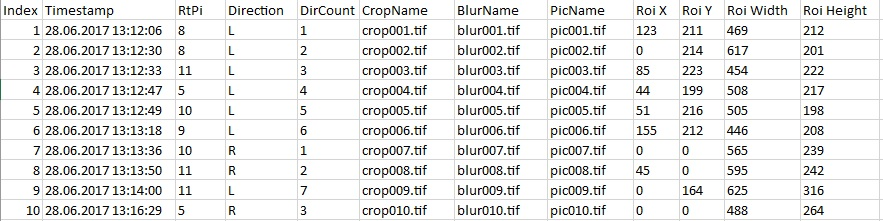
\includegraphics[width=1\textwidth]{Resultate/FeatureVector.jpg} 
  \caption{Feature Vektor eines einzelnen Gerätes.}
  \label{bFVec}
\end{figure}

\subsubsection{Zählen}
Mithilfe eines einzelnen Gerätes kann an den Aufstellpunkten die Anzahl der vorbeifahrenden Verkehrsteilnehmer gezählt werden. An jedem der Aufstellpunkte erhält somit der Bediener eine Anzahl der Verkehrsteilnehmer welche in das Gebiet fahren und welche sich aus dem Gebiet heraus bewegen. Jedes dieser gezählten Verkehrsteilnehmer erhält zugleich eine vorlaufende Nummer, sowie einen Zeitstempel und eine Fahrtrichtung.

\subsubsection{Kategorisieren}
Jedes Einzelgerät ist ebenso im Stande die vorbeifahrenden Verkehrsteilnehmer in vordefinierte Kategorien einzuteilen. Dabei wird die Anzahl an Pixel welche sich bewegen gezählt und durch dies eine quantitative Kategorisierung in drei Kategorien zerlegt werden. Wie in \fref{bNachverarbeitung} in Spalte drei zusehen ist werden die Kategorien in NV, 1 und 2 eingeteilt. NV sind Verkehrsteilnehmer welche kleiner als ein Auto sind. Die 1 gibt an, dass es sich um ein Auto handelt und 2 sind dann grössere Verkehrsteilnehmer.

\subsubsection{Geschwindigkeitserkennung}
Um den Verkehrsfluss darstellen zu können, wird die momentane Geschwindigkeit des Verkehrsteilnehmers verwendet. Die Geschwindigkeit wird aus zwei aufeinanderfolgenden Frames extrahiert. Dabei wird der Positionsunterschied der Fahrzeuge auf den Frames verwendet um die Geschwindigkeit zu berechnen. Um die Geschwindigkeit berechnen zu können, wurde eine Referenzmessung durchgeführt, bei welcher zwischen zwei Positionsunterschieden, eine Pixelverschiebung von 58 Pixel pro km/h gemessen wurde. Nun kann durch einfache Schlussrechnung die Geschwindigkeit der Verkehrsteilnehmer berechnet werden. Dabei wird der Positionsunterschied, in Pixel, durch die Referenzmessung geteilt, und so erhält man die Geschwindigkeit der Fahrzeuge. Auf der \fref{bNachverarbeitung} in Spalte sechs, sind die berechneten Geschwindigkeiten zu sehen und mit einem freiwählbaren Farbcode, zur besseren Veranschaulichung, markiert. Um die Geschwindigkeitsverteilung noch besser darzustellen, wurden diese wie in \fref{bGeschwDiagramm} in einem Diagramm veranschaulicht. Der grösste Teil der Verkehrsteilnehmer hielt sich beinahe an die 50km/h Grenze im Dorf, jedoch wurden Geschwindigkeiten weit über diesen gemessen welche auch gefahren werden, da der Messpunkt am Ende des Dorfes liegt.

\begin{figure}[H]
  \centering
  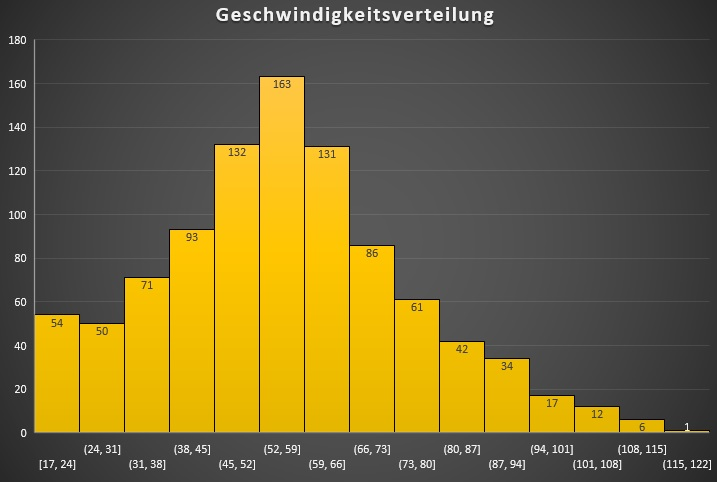
\includegraphics[width=0.6\textwidth]{Resultate/GeschwDiagramm.jpg} 
  \caption{Diagramm der Geschwindigkeitsverteilung auf einer 50er Straße am Ende eines Dorfes.}
  \label{bGeschwDiagramm}
\end{figure}


\begin{figure}[H]
  \centering
  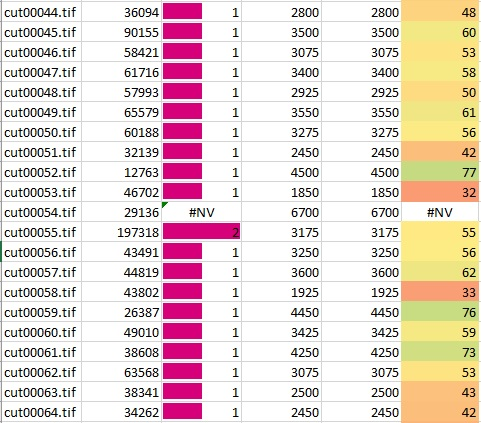
\includegraphics[width=0.6\textwidth]{Resultate/Nachverarbeitung.jpg} 
  \caption{Tabelle des nachverarbeiteten Feature Vektor.}
  \label{bNachverarbeitung}
\end{figure}